\let\negmedspace\undefined
\let\negthickspace\undefined
\documentclass[journal]{IEEEtran}
\usepackage[a5paper, margin=10mm, onecolumn]{geometry}
%\usepackage{lmodern} % Ensure lmodern is loaded for pdflatex
\usepackage{tfrupee} % Include tfrupee package

\setlength{\headheight}{1cm} % Set the height of the header box
\setlength{\headsep}{0mm}     % Set the distance between the header box and the top of the text

\usepackage{gvv-book}
\usepackage{gvv}
\usepackage{cite}
\usepackage{amsmath,amssymb,amsfonts,amsthm}
\usepackage{algorithmic}
\usepackage{graphicx}
\usepackage{textcomp}
\usepackage{xcolor}
\usepackage{txfonts}
\usepackage{listings}
\usepackage{enumitem}
\usepackage{mathtools}
\usepackage{gensymb}
\usepackage{comment}
\usepackage[breaklinks=true]{hyperref}
\usepackage{tkz-euclide} 
\usepackage{listings}
% \usepackage{gvv}                                        
\def\inputGnumericTable{}                                 
\usepackage[latin1]{inputenc}                                
\usepackage{color}                                            
\usepackage{array}                                            
\usepackage{longtable}                                       
\usepackage{calc}                                             
\usepackage{multirow}                                         
\usepackage{hhline}                                           
\usepackage{ifthen}                                           
\usepackage{lscape}
\begin{document}

\bibliographystyle{IEEEtran}
\vspace{3cm}

\title{NCERT-9.5.13}
\author{EE24BTECH11065 - Spoorthi yellamanchali
}
% \maketitle
% \newpage
% \bigskip
{\let\newpage\relax\maketitle}

\renewcommand{\thefigure}{\theenumi}
\renewcommand{\thetable}{\theenumi}
\setlength{\intextsep}{10pt} % Space between text and floats


\numberwithin{equation}{enumi}
\numberwithin{figure}{enumi}
\renewcommand{\thetable}{\theenumi}


\textbf{Question:}
\\
Find the solution of the following differential equation:
\begin{align*} 
\left[ x \sin^2 \left( \frac{y}{x} \right) - y \right] dx + x \, dy = 0; \quad y = \frac{\pi}{4} \text{ when } x = 1 
\end{align*}
\\
\textbf{ Theoretical Solution: }
\\
From the question,
\begin{align} 
\frac{dy}{dx} = \frac{y}{x} - \sin^2{\frac{y}{x}};
\end{align} 
Let $t = \frac{y}{x}$,then, 
\begin{align}
    \frac{dy}{dx} = x\frac{dt}{dx} + t
\end{align}
On substituting the value of $\frac{dy}{dx}$ in the equation $\brak{0.1}$,we get,
\begin{align}
x\frac{dt}{dx} = -\sin^2{t};
-\cosec^2{t}\ dt = \frac{dx}{x};
\end{align}
On integrating on both sides,
\begin{align}
     \int -\cosec^2{t}\ dt = \int \frac{dx}{x};\\
     \cot{t} = \ln{x} + c;\\
     \cot{\frac{y}{x}} = \ln{x} + c
\end{align}
On Substituting given initial conditions in the equation $\brak{0.6}$\\
we get $c = 1$.
\begin{align}
\therefore y = x\cot^{-1}{(\ln{x} + 1)}
\end{align}
\textbf{Solution by the method of finite differences:}
\\
The finite difference method is a numerical technique for solving differential equations by approximating derivatives with differences.\\
The first forward difference approximation of the derivative of $f(x)$ at $x$ is given by: \\
%This is forward difference, there are variations like backward difference, central differences also...

\begin{align}
    \frac{dy}{dx}=\frac{f(x+h)-f(x)}{h}      
\end{align}
On taking the given point on the curve as the initial conditions $\brak{x_0,y_0}$,we can get ,
\begin{align}
    x_1 = x_0 + h;
\end{align}
And from the above equation,we can get
\begin{align}
  y_1 = y_0 + h\brak{\frac{dy}{dx}|_{x=x_0}}   
\end{align}
we know that our derivative is given by:\\
\begin{align}
    \frac{dy}{dx} = \frac{y}{x} - \sin^2{\frac{y}{x}};
\end{align}
On substituting the expression of the derivative in equation $\brak{0.11}$, we get
\begin{align}
    y_1 = y_0 + h\brak{\frac{y_0}{x_0} - \sin^2{\frac{y_0}{x_0}}} 
\end{align}
On assuming a value for $h$ which is close to zero  and by substituting the values of $x_0$ and $y_0$ in the above equations we get the point $\brak{x_1,y_1}$. \\
what we have essentially done above is, obtaining a point which is very close to the initial point along the direction of derivative at that point.\\
similarly we get,
\begin{align}
    x_n = x_{n-1} + h ;\\
y_n = y_{n-1} + h\brak{\frac{y_{n-1}}{x_{n-1}} - \sin^2{\frac{y_{n-1}}{x_{n-1}}}}
\end{align}
we can obtain points on the curve by using the above expressions for $y_n$ and $x_n$\\
 $\therefore$ we can plot the curve by the points obtained.
\begin{figure}[h!]
   \centering
   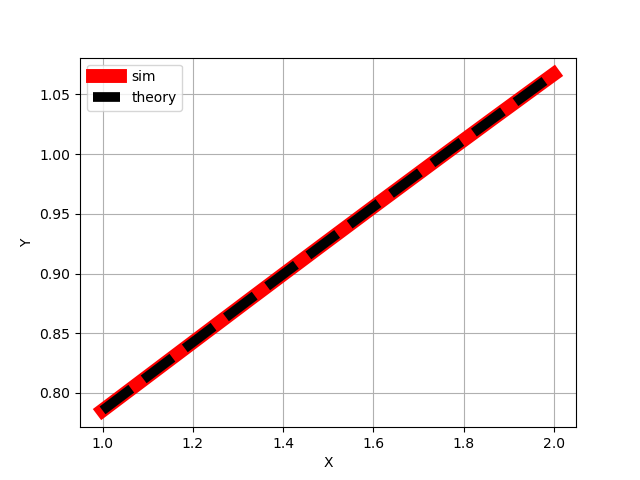
\includegraphics[width=0.75\columnwidth]{figures/Figure_1.png}
\end{figure}
\end{document}


